% This is file JFM2esam.tex
% first release v1.0, 20th October 1996
%       release v1.01, 29th October 1996
%       release v1.1, 25th June 1997
%       release v2.0, 27th July 2004
%       release v3.0, 16th July 2014
%   (based on JFMsampl.tex v1.3 for LaTeX2.09)
% Copyright (C) 1996, 1997, 2014 Cambridge University Press

\documentclass{jfm}
\usepackage{graphicx}
%\usepackage{epstopdf, epsfig}
\usepackage{physics}

\usepackage{enumitem,amssymb}
\newlist{todolist}{itemize}{2}
\setlist[todolist]{label=$\square$}
\usepackage{pifont}
\newcommand{\cmark}{\ding{51}}%
\newcommand{\xmark}{\ding{55}}%
\newcommand{\done}{\rlap{$\square$}{\raisebox{2pt}{\large\hspace{1pt}\cmark}}%
\hspace{-2.5pt}}
\newcommand{\wontfix}{\rlap{$\square$}{\large\hspace{1pt}\xmark}}

\newtheorem{lemma}{Lemma}
\newtheorem{corollary}{Corollary}

\newcommand{\cz}{c_{\zeta}}
\newcommand{\cs}{c_{\psi}}
\newcommand{\ct}{c_{\theta}}
\newcommand{\cu}{c_u}
\newcommand{\css}{c_{\psi \psi}}
\newcommand{\csz}{c_{\psi \zeta}}
\newcommand{\czs}{c_{\zeta \psi}}
\newcommand{\czz}{c_{\zeta \zeta}}
\newcommand{\ctz}{c_{\theta \zeta}}
\newcommand{\czt}{c_{\zeta \theta}}
\newcommand{\ctt}{c_{\theta \theta}}
\newcommand{\cst}{c_{\psi \theta}}
\newcommand{\cts}{c_{\theta \psi}}
\newcommand{\Rayleigh}{\mbox{\textit{Ra}}}  % Rayleigh number
\newcommand{\Pra}{\mbox{\textit{Pr}}}  % Prandtl number


\shorttitle{CE2 Busse Annulus}
\shortauthor{J. S. Oishi, K. J. Burns, J. B. Marston, S. M. Tobias}

\title{Direct Statistical Simulation of the Busse Annulus}

\author{Jeffrey S. Oishi\aff{1}
  \corresp{\email{joishi@bates.edu}},
  Keaton J. Burns\aff{2,3},
  J. B. Marston\aff{4},
 \and Steven M. Tobias\aff{5}}

\affiliation{\aff{1}Department of Physics \& Astronomy, Bates College,
Lewiston, ME 04240, USA
\aff{2} Department of Mathematics, Massachusetts Institute of Technology, Cambridge, MA 02138 USA
\aff{3} Center for Computational Astrophysics, Flatiron Institute, New York, NY 10010, USA
\aff{4} Department of Physics, Brown University, Providence, RI 02912, USA
\aff{5} Department of Applied Mathematics, University of Leeds, Leeds LS2 9JT, UK
}

\begin{document}

\maketitle

\begin{abstract}
We consider direct statistical simulation (DSS) of a paradigm system of convection interacting with mean flows. In the Busse Annulus model zonal jets are generated through the interaction of convectively driven turbulence and rotation; non-trivial dynamics including the emergence of multiple jets and bursting 'predator-prey' type dynamics can be found. We formulate the DSS by expanding around the mean flow in terms of equal-time cumulants and arrive at a closed set of equations of motion for the cumulants. Here, we present results using an expansion terminated at the second cumulant (CE2); it is fundamentally a quasi-linear theory.
We focus on a particular cases including bursting and bistable multiple jets and demonstrate that CE2 can reproduce the results of direct numerical simulation if particular attention is given to symmetry considerations. 
%in which the direct numerical simulation yields an initial three-jet solution that is unstable to a two-jet solution.
%Interestingly, CE2 predicts a stable three-jet solution, though we find that by biasing the initial conditions to favor certain symmetries, CE2 reproduces the DNS results.
\end{abstract}

\begin{keywords}
\end{keywords}

\section{Introduction}
\label{sec:intro}

Moved from abstract: Turbulent systems generate and interact with mean flows in a wide variety of natural systems.
Understanding the nature of these interactions, particularly for systems far from equilibrium, remains a key problem for the description of large-scale flows on planets and stars.
The fundamental problem in studying such systems via direct numerical simulation (DNS) is the expense of the calculations owing to the vast range of spatial and temporal scales that need to be described. 
One way to make progress is to study the statistics of the flow rather than detailed flow variables themselves. However, these systems are often inhomogeneous and strongly anisotropic, and such a statistical description should respect this.

Rotation is a hallmark of geophysical and astrophysical fluid dynamics.
Through the breaking of reflectional symmetry, rotating systems are known to generate mean flows such as zonal jets; examples of which include the bands on Jupiter, the jet stream on Earth and the differential rotation in stars.
It is common that the production of these jets is driven by rotating convection.

%Understanding the interaction between turbulence and mean flows remains a major challenge as such systems are often at extreme parameters inaccessible to direct numerical simulation (DNS).

Here, we explore one particular system, the Busse Annulus, using the CE2 formulation of direct statistical simulation.
CE2 is a cumulant expansion truncated at second order and is fundamentally quasilinear.
Our recent work \citep{2018RSPSA.47480422T} has shown that in direct simulation, the generalized quasilinear approximation (GQL) outperforms QL models at all parameter values explored.

The Busse annulus model considers convection in a duct with slanted ends leading to a topographic $\beta$ effect.
This system present an important challenge for CE2, as it is possesses a linear instability which is known to host multiple solutions at modest Rayleigh numbers \citep{bh1993}.
How does a quasilinear statistical theory fare when faced with multiple potential solution basins?
In particular, we investigate the sensitivity of CE2 to initial conditions for a case with multiple solution branches.

\section{Model Equations, Formulation, Parity and Numerical Methods}
\label{sec:model-eqations}

We consider the equations for the Busse annulus \citep[e.g.][]{bh1993, rj2006}
\begin{equation}
  \label{eq:zeta_eom}
  \pdv{\zeta}{t} + J(\psi, \zeta) - \beta \pdv{\psi}{x} = -\frac{\Rayleigh}{\Pran} \pdv{\theta}{x} -C |\beta|^{1/2} \zeta + \laplacian{\zeta}
\end{equation}
where $\psi$ is the streamfunction, $(u,v) = (-\pdv*{\psi}{y}, \pdv*{\psi}{x})$, and the $z$-component of vorticity is 
\begin{equation}
  \label{eq:zeta_def}
  \zeta = \laplacian{\psi}.
\end{equation}
$J(A, B) = \pdv*{A}{x}\pdv*{B}{y} - \pdv*{A}{y}\pdv*{B}{x}$ is the Jacobian. 
The temperature perturbation from a linear background state is given by $\theta$ and evolves according to
%
\begin{equation}
  \label{eq:theta}
  \pdv{\theta}{t} + J(\psi, \theta) = -\pdv{\psi}{x} + \frac{1}{\Pran} \nabla^2 \theta.
\end{equation}
The system is governed by four dimensionless parameters, $\beta$, $C$, $\Pran = \nu/
\kappa$, and $\Rayleigh = \alpha g \Delta T d^3/\nu \kappa$.

The CE2 formulation is implemented using a zonal average, 
\begin{equation}
\langle f(x,y) \rangle = \frac{1}{L_x} \int_0^{L_x} f(x,y) dx
\end{equation}
to split all dynamical variables into mean and fluctuating components,
\begin{equation}
    f(x,y,t) = \langle f \rangle + f'.
\end{equation}
We then derive evolution equations for the first cumulants $\cz(y) = \langle \zeta \rangle $ and $\ct(y) = \langle \theta \rangle$ and the second cumulants 
\begin{equation}
    \ctt(\xi,y_1,y_2) = \langle \theta^\prime(x_1,y_1) \theta^\prime(x_2,y_2) \rangle
\end{equation}
with $\xi = x_1 - x_2$.
Similar definitions are used for the second cumulants $\czz$, $\ctz$, and $\czt$. 
Cumulants involving $\psi$ and $\zeta$ are related by differential operators \citep{2013PhRvL.110j4502T}.
Because the equations require both $\psi$ and $\zeta$ cumulants, we solve for $\cs$, $\ct$, $\css$, $\cts$, $\cst$, and $\ctt$, though we write equations in terms of $\zeta$ cumulants.

The  dynamical equations for the cumulants are given by
\begin{equation}
  \label{eq:cz}
  \pdv{\cz}{t} = - \qty(\pdv{y_1} + \pdv{y_2}) \pdv{\csz}{\xi}\eval_{\xi \to 0}^{y_1 \to y_2} - C |\beta|^{1/2} \cz + \pdv[2]{\cz}{y_1},
\end{equation}

\begin{equation}
  \label{eq:czz}
  \begin{split}
    \pdv{\czz}{t} &= \pdv{\cs}{y_1} \pdv{\czz}{\xi} - \qty(\pdv{\cz}{y_1} - \beta) \pdv{\csz}{\xi} - \pdv{\cs}{y_2} \pdv{\czz}{\xi}  + \qty(\pdv{\cz}{y_2} - \beta) \pdv{\czs}{\xi}\\
    &+ \frac{\Rayleigh}{\Pran} \qty(\pdv{\czt}{\xi} -  \pdv{\ctz}{\xi}) - 2C |\beta|^{1/2} \czz + (\nabla_1^2 + \nabla_2^2) \czz,    
  \end{split}
\end{equation}

\begin{equation}
  \label{eq:ct}
  \pdv{\ct}{t} = - \qty(\pdv{y_1} + \pdv{y_2}) \pdv{\cst}{\xi} \eval_{\xi \to 0}^{y_1 \to y_2} + \frac{1}{\Pran} \pdv[2]{\ct}{y_1}l,
\end{equation}

\begin{equation}
  \label{eq:ctt}
\begin{split}
  \pdv{\ctt}{t} &= \pdv{\cts}{\xi} - \pdv{\cst}{\xi} + \left(\pdv{\cs}{y_1} - \pdv{\cs}{y_2}\right)\pdv{\ctt}{\xi} + \pdv{\ct}{y_2}\pdv{\cts}{\xi} - \pdv{\ct}{y_1}\pdv{\cst}{\xi}\\
&  + \frac{1}{\Pran}(\nabla_1^2 + \nabla_2^2) \ctt,
\end{split}
\end{equation}
and
\begin{equation}
  \label{eq:ctz}
  \begin{split}
    \pdv{\ctz}{t} &= \qty(\pdv{\cs}{y_1} - \pdv{\cs}{y_2}) \pdv{\ctz}{\xi} - \qty(1 + \pdv{\ct}{y_1}) \pdv{\csz}{\xi} + \qty(\pdv{\cz}{y_2} - \beta) \pdv{\cts}{\xi}\\
    &  - C |\beta|^{1/2} \ctz + \frac{1}{\Pran} \nabla_1^2 \ctz + \nabla_2^2 \ctz.
  \end{split}
\end{equation}
Other second cumulant terms can be calculated from symmetry considerations.
% This could be calculated using symmetry, $\czt(y_1, y_2, \xi) = \ctz(y_2, y_1, -\xi)$.
% However, because we use IMEX timestepping and such symmetry operations can only be applied at the end of a timestep, this would mean that $\czt$ would not be updated during the implicit step.
% Instead, we solve an equation for $\czt$ which is identical to equation~(\ref{eq:ctz}) with $x_1,y_1$ and $x_2, y_2$ swapped.

We solve the system subject to impenetrable, stress-free boundary conditions in the $y$ dimension; it is periodic in $x$. 
This means that $\theta$, $\zeta$, and $\psi$ all have odd parity.
The action of the zonal average preserves the parity, so we discretize the first cumulants using a $\sin$ series in $y$. 
The second cumulants are discretized on $\sin$ series in $y_1$ and $y_2$ and a Fourier basis in $x$.
All variables in the DNS simulations are discretized on $\sin$ series in $y$ and Fourier bases in $x$.

We use \emph{Dedalus} \citep{2020PhRvR...2b3068B} to solve both the direct equations (\ref{eq:zeta_eom} - \ref{eq:theta}) and the CE2 model equations, (\ref{eq:cz})-~(\ref{eq:ctz}).
For the CE2 equations, we use RK222 timestepping with all terms evaluated explicitly.
We have found this to be more stable than the typical approach of using implicit-explicit (IMEX) timesteppers with implicit integration for linear terms and explicit integration non-linear terms.
The DNS simulations use the SBDF2 IMEX scheme with linear terms implicit.

\section{Results}
\label{sec:results}








Minimally, we begin each CE2 simulation using one of two extreme initial conditions: \emph{maximum ignorance}, in which we assume a completely uncorrelated $\ctt$ and all other fields zero, and \emph{maximum knowledge}, in which we initialize all fields using cumulants calculated from a DNS solution. This allows us to evaluate CE2's ability to both \emph{find} solutions and \emph{continue} solutions already known. We also begin some solutions with biased initial conditions that ensure solutions are not trapped in symmetry subspaces.

In order to facilitate comparison with previous work, we adapt the same run naming scheme as in \citet{2018RSPSA.47480422T}.

\begin{table}
  \begin{center}
\def~{\hphantom{0}}
  \begin{tabular}{lcccccl}
    Run & $\beta$ & $\Rayleigh$ & $C$ & DNS Resolution & CE2 Resolution & Comment \\[3pt]
    A  & $2.8\times 10^3$ & $7.6 \times 10^4$   & $0$ & $256 \times 64$ & $32^3$ & Two-jet \\
    B  & $7.07\times 10^5$ & $10^8$ & $0.316$ & $512 \times 256$ & $128 \times 64$ & Seven-jet  \\
    C  & $5\times 10^5$ & $8\times 10^7$ & $0$ & $512 \times 256$ & $256 \times 64$ & three-jet $\to$ two-jet bursting \\
    R  & $3.16\times 10^5$ & $4\times 10^7$ & $0.316$ & $256 \times 64$ & $128\times 64^2$ & Five-jet\\
    Rb  & $3.16\times 10^5$ & $4\times 10^7$ & $0.316$ & - & $128\times 64^2$ & CE2 3-jet initial bias\\
  \end{tabular}
  \caption{Runs}
  \label{tab:runs}
  \end{center}
\end{table}

\subsection{Run A: 2 Jet/3 Jet solutions}
\label{sec:hov}

\begin{figure}
  \centering
  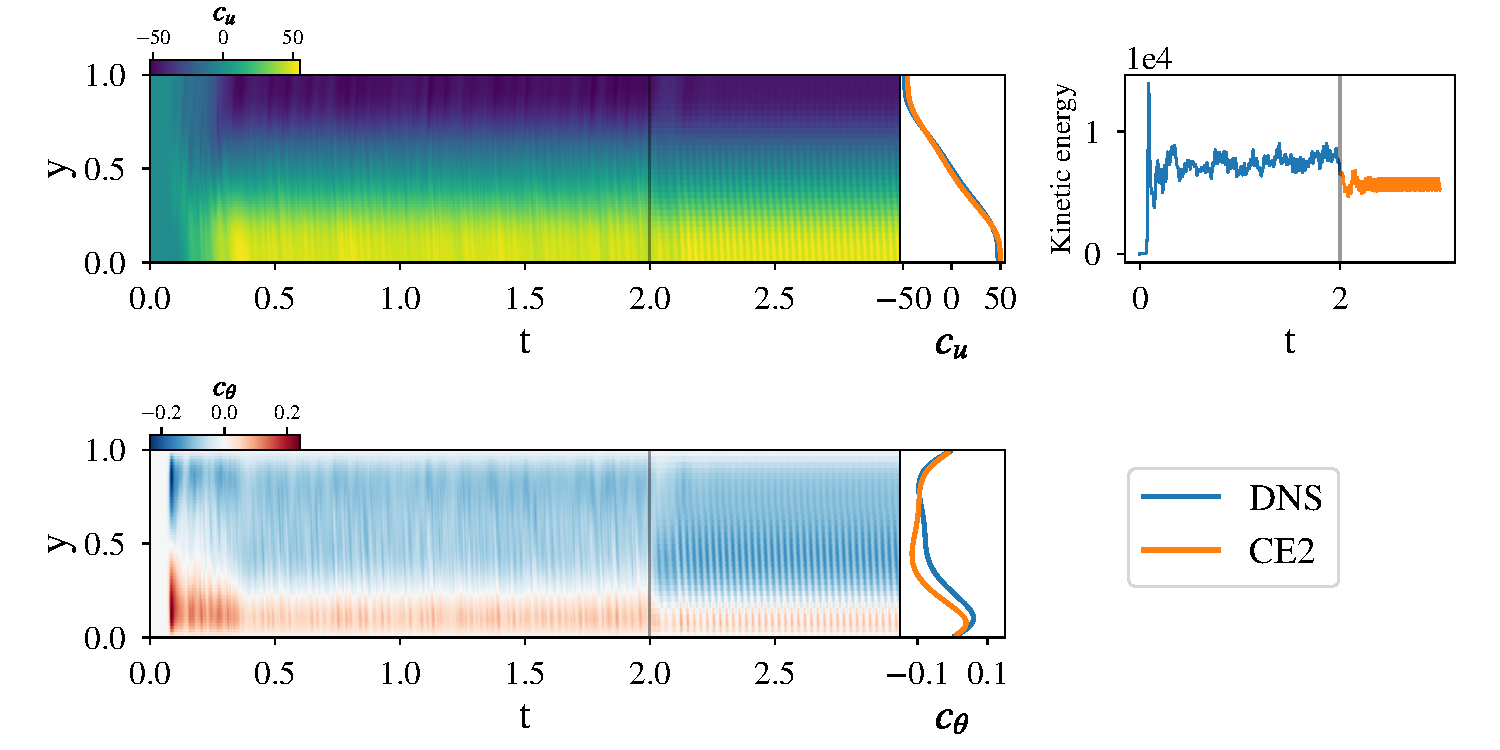
\includegraphics[width=\textwidth]{../../figs/run_A_fig.pdf}
  \caption{Left: hovmoller diagrams of first cumulants $\cu$ (upper), $c_\theta$ (lower) from run A started in DNS and continued at $t=2$ with DNS. Middle: time-averaged first cumulants as a function of $y$ for both CE2 and DNS averaged over $1 \le t \le 2$ for DNS and $2 \le t \le 3$ for CE2. Right: total kinetic energy.}
  \label{fig:run_A}
\end{figure}
%DESCRIPTION OF FIGURE 1.
%\begin{itemize}
%    \item CASE A: DNS 3 jet solution turns into 2 jet solution. Probable co-existence.
%    \item CE2
%    \begin{itemize}
%        \item If started with maximum ignorance get 3 jet solution (this has a symmetric temperature).
%        \item If solution is biased by providing correct symmetry to initial cumulants then you can get 2 jet solution.
%        \item If solution starts with maximum knowledge (i.e. from end state of DNS) then can reprpduce form of the solution including asymmetry in mean temperature
%    \end{itemize}
%\end{itemize}

The first case we consider (case A) exhibits relatively simple dynamics in DNS. Started from random initial conditions, the driven convection interacts with the $\beta$-effect to drive large-scale zonal flows (jets). These takes the form of one prograde and one retrograde jet as shown in the solutions for the mean zonal velocity $\langle u \rangle(y, t)$ and mean temperature $\langle \theta\rangle(y,t) $ in Figure~\ref{fig:run_A} 
We begin by comparing the time evolution of the zonal average jets,  in DNS and CE2 simulations.
Started from random initial conditions, however, CE2 evolves to a 3-jet solution, which is symmetric about the midplane ($y=0.5$). These results are similar to the strictly quasilinear run in \citet{2018RSPSA.47480422T}, which also produces a 3-jet solution; an unsurpring result given that 
 CE2 is fundamentally a quasi-linear theory, this is unsurprising (Generalised Quasilinear Solutions do however yield the correct number of jets). At these parameters it has been demonstrated that  there is hysteresis between 2-jet and 3-jet solutions known, but that 3-jet solutions may be unstable to perturbations that break shift-reflect symmetry \citep{bh1993}. Using Dedalus, we ran a DNS with initial conditions that respect this symmetry. Owing to our highly accurate spectral methods, the 3-jet solutions could remain stable in DNS.

Interesting solutions emerge, however, when the CE2 solution is biased 
 by initializing the first cumulant of the x-velocity, $\cu$ to
\begin{equation}
  \label{eq:bias}
  \cu(t=0, y_0) = A_0 \left( \lambda cos(2\pi/L_y y_0) + (1-\lambda) cos (\pi/L_y y_0)\right).
\end{equation}
The first term is odd about the center of the domain, while the second is even; we can solve for $c_\psi$ given $\cu$ for our initial conditions.
%\footnote{note that both have even parity with respect to the boundary connditions, as required by the boundary conditions}.
%We use the linear boundary value solver in \emph{Dedalus} to solve for 
$c_\psi$ given $\cu$
%, and use this as an additional initial condition for $c_\psi$; in our unbiased simulations, $c_\psi(t=0) = 0$.

%If the linear growth rate explanation is correct, then one would expect that for $\lambda \ll 1$ would lead the CE2 results to pick up the 2-jet solutions.
%They do not.
Using a substantially biased initial condition, CE2 \emph{is} capable of sustaining a 2-jet solution
%by biasing our simulation with $\lambda = 1$ and giving a substantial initial amplitude $A_0 = 40$, the CE2 results do reveal the 2-jet solution, and they 
that saturates at an amplitude comparable with the DNS results. This strongly suggests that the transition from 3 to 2 jets is the product of a subcritical, non-linear transition mediated by eddy-eddy $\to$ eddy interactions excluded from CE2 as well as our previous quasilinear results.
Regardless, this solution remains a fixed point of the CE2 system, suggesting that the \emph{selection} of a given multi-jet solution is distinct from its \emph{maintenence}.
This hypothesis is supported by our "maximal knowledge" solution where the CE2 solution is initialised with the cumulants calculated from the saturated state of the DNS run (see Figure~\ref{fig:run_A}). CE2 is certainly capable of maintaining the form of these fully nonlinear solutions (even maintaining the slight asyymetry in the temperature distribution) even though the EENL term is missing from the system.


\begin{figure}
    \centering
    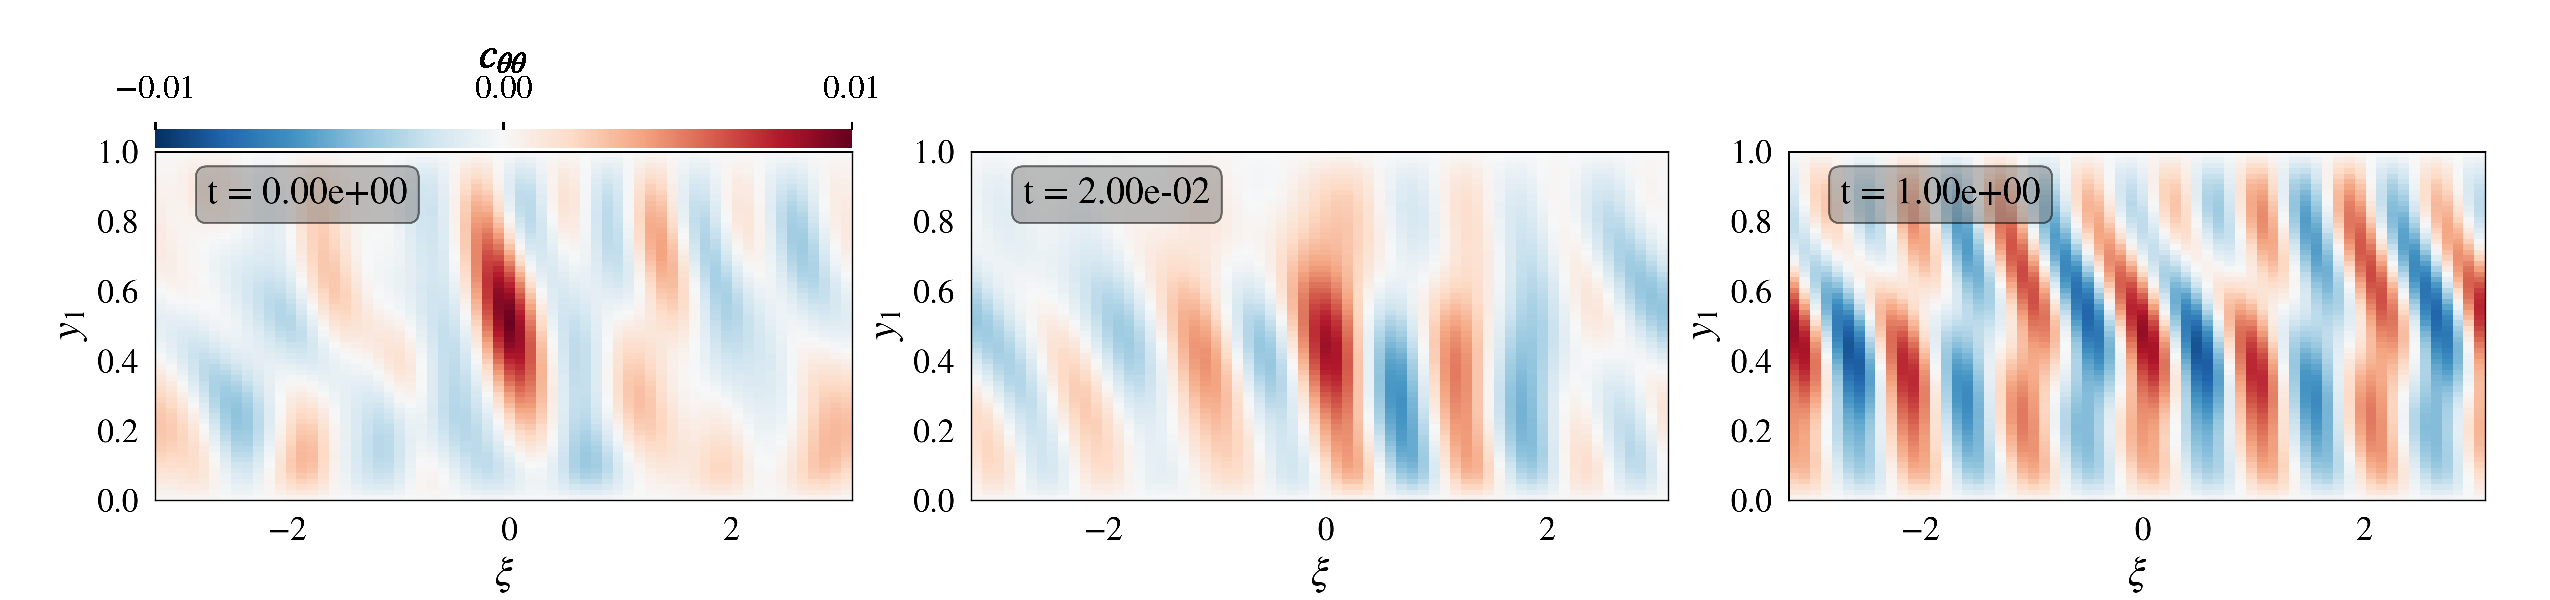
\includegraphics[width=\textwidth]{../../figs/run_A_decoherence.pdf}
    \caption{$\ctt(\xi, y_1, y_2 = 0.5)$ as a function of time for run A with ``maximum knowledge'' initial conditions selected from the output of DNS. Note that the initial, tightly peaked $\ctt$ from DNS (left most panel) quickly delocalizes and reverts to the overemphasis of long-range correlations characteristic of CE2.}
    \label{fig:run_A_decoherence}
\end{figure}
%DESCRIPTION OF FIGURE 2.
%\begin{itemize}
%    \item CASE A: Starting from DNS the first cumulant is fairly well reproduced.
%    \item What happens to the second cumulant?
%    \begin{itemize}
%        \item Starts off fairly localised. Eddy/Eddy interactions are important in maintaining the locality of the correlations.
%        \item As calculation proceeds correlations delocalise
%        \item Eventually the second cumulant is very delocalised and has a wave-like form. Interacting thermally driven Rossby waves.
%    \end{itemize}
%\end{itemize}

The degree of success of the quasilinear CE2 models can be investigated at greater depth by comparing the second cumulants. Figure~\ref{fig:run_A_decoherence} shows the evolution of the second cumulant $\ctt(\xi, y_1, y_2 = 0.5)$ under CE2 for the solution started from the saturated state of a DNS calculation. The figure shows that this covariance of the DNS is fairly localised in space. We hypothesise that EENL interactions are important in maintaining the locality of these correlations. This hypothesis is validated by the fact that the correlations delocalise in space as the calculation progresses. Eventually the second cumulant is very delocalised and has a wave-like form. The long-range teleconnections a typical of (in this case) thermally driven Rossby waves interacting with a mean flow; the quasilinear nature of CE2 leads to this interaction being favoured.

\subsection{Multiple Jet Solutions}
\begin{figure}
  \centering
  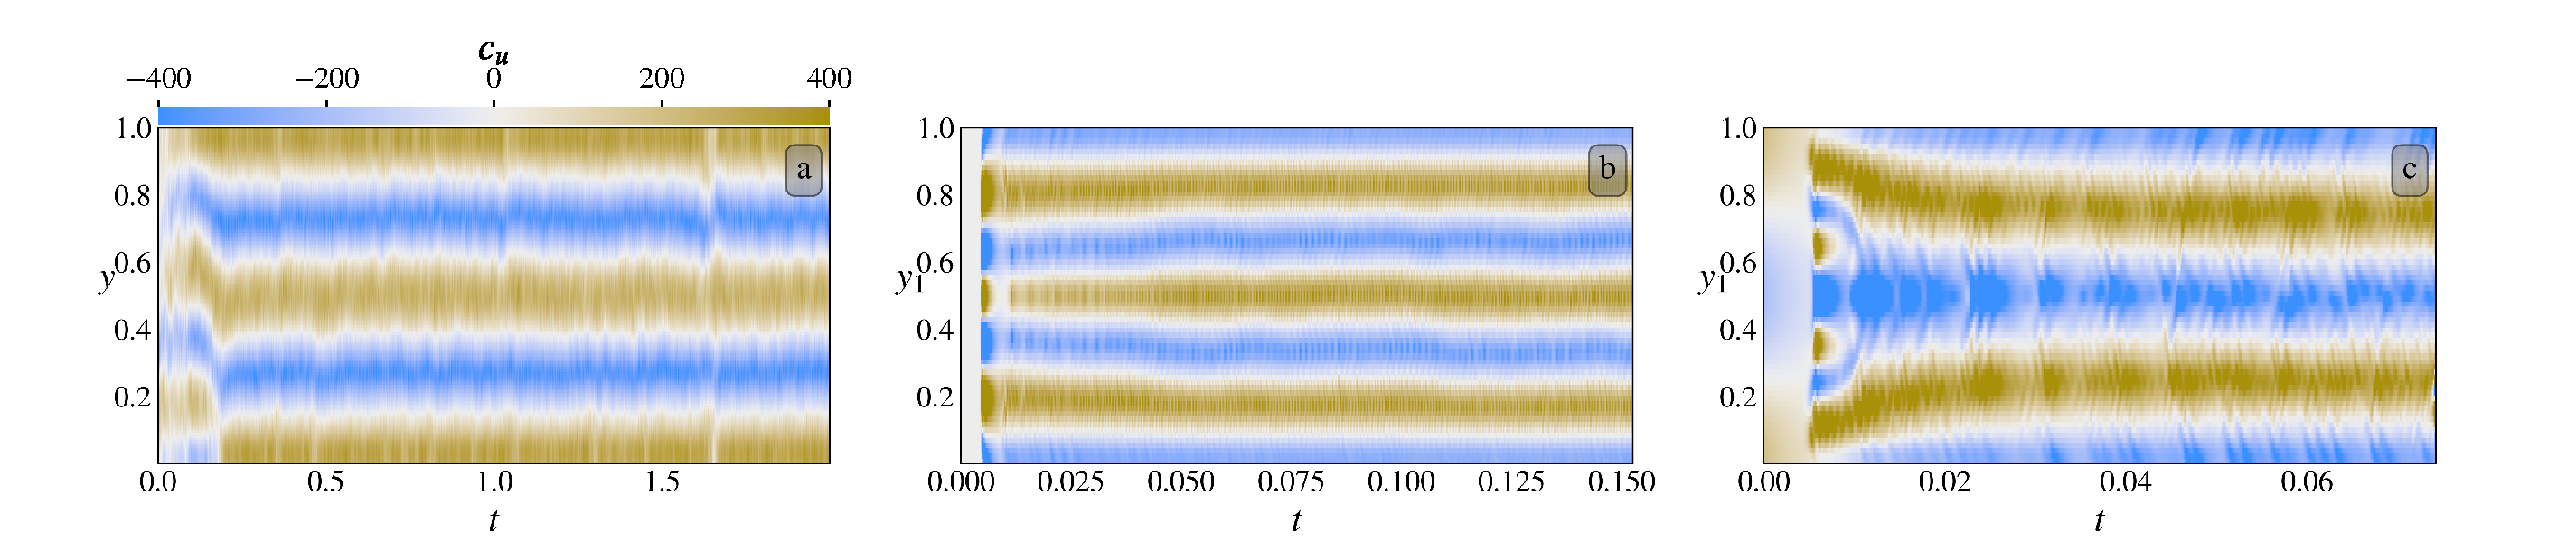
\includegraphics[width=\textwidth]{../../figs/run_R_S_hov_cu_dns_ce2.pdf}
  \caption{Hovmoller diagrams of run R in DNS (a),  run R in CE2 (b), and run Rb in CE2. In panel (b), the first cumulant $\cu$ is zero at $t = 0$. CE2 picks up a stable 7-jet solution. In panel (c), the CE2 initial condition is biased with a 3-jet solution. In this case, CE2 latches on to the correct 5-jet solution.}
  \label{fig:hov_run_R}
\end{figure}

\begin{figure}
  \centering
  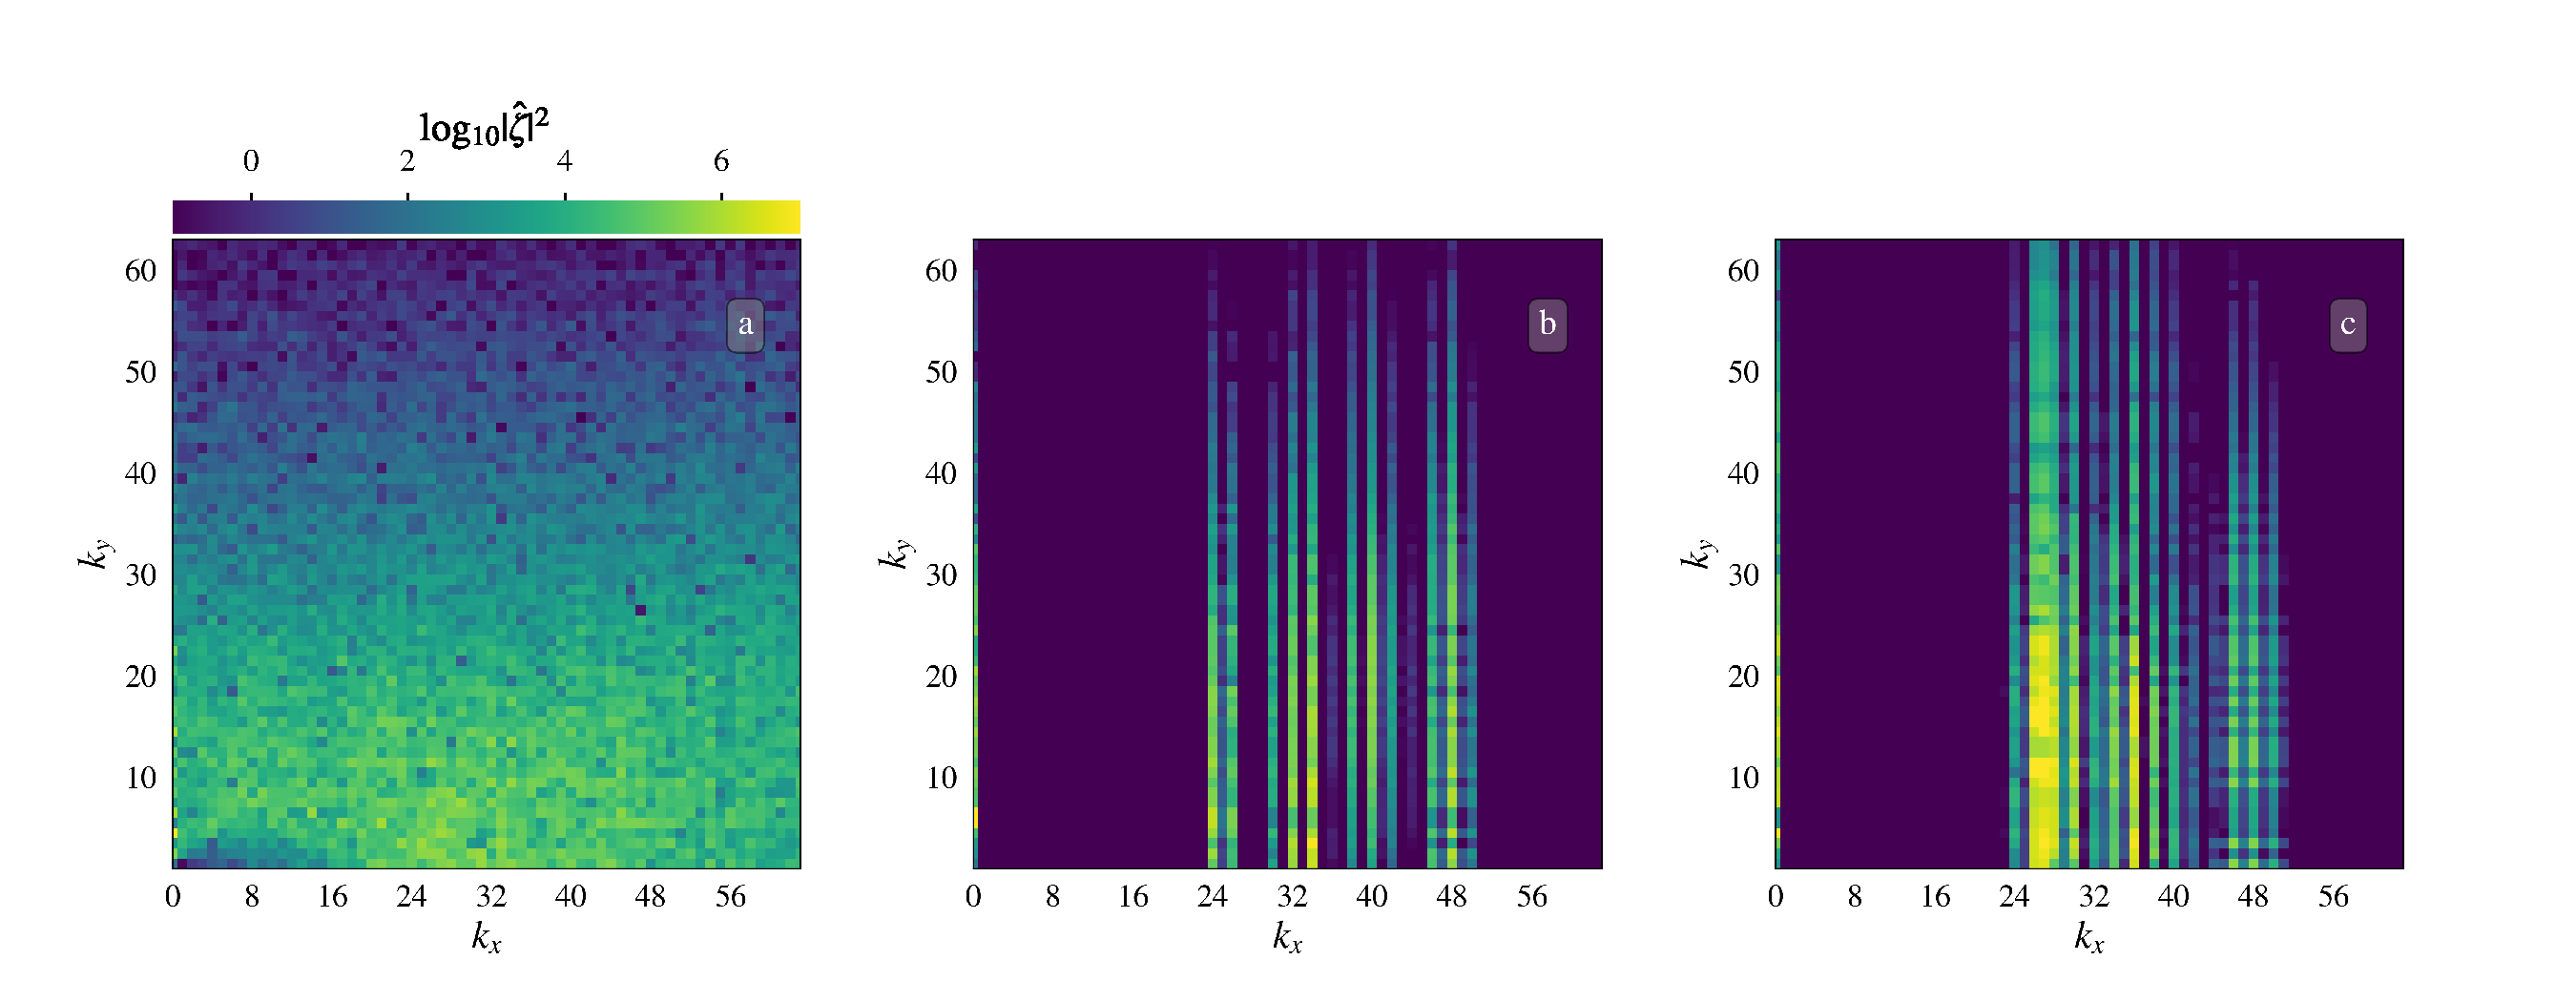
\includegraphics[width=\textwidth]{../../figs/power_spectra_zeta_dns_run_R.pdf}
  \caption{NOTE: emphasize the DNS panel shows energy is distributed across many $k$ showing that eddy-eddy NL is very important, but that doesn't seem to affect mean too badly. Perhaps just leading to dissipation? From left to right: power spectra of $\zeta$ in run R from a) DNS, b) unbiased CE2 c) CE2 biased with initial 3 jet solution.}
  \label{fig:power_spec_S}
\end{figure}
%DESCRIPTION OF FIGURE 4.
%\begin{itemize}
%    \item CASE R: DNS is a five jet solution (left panel shows full spectrum)
%    \item CE2? 
%    \begin{itemize}
%        \item Unbiased (max ignorance) gives a 7 jet solution. Spectrum shows certain symmetry in wavenumbers
%        \item biased (min ignorance). Spectrum different
%    \end{itemize}
%\end{itemize}
%DESCRIPTION OF FIGURE 3.
%\begin{itemize}
%    \item CASE R: DNS is a five jet solution
%    \item CE2? 
%    \begin{itemize}
%        \item Unbiased (max ignorance) gives a 7 jet solution
%        \item If given a 3 jet solution manages to find a 5 jet solution (via 7 jets)
%        \item If given end of DNS presumably manages to carry it on.
%    \end{itemize}
%\end{itemize}

Parameters may also be selected that yield multiple jets. Case R, for which the DNS is shown in Figure~\ref{fig:hov_run_R}(a) is such a case. Here, after an initial transient that takes the form of a six jet solution, a jet merging leads to the solution settling down into a five jet solution. For this DNS solution the second cumulant is very localised, which is suggested by the broad power spectrum of the DNS shown in Figure~\ref{fig:power_spec_S}(a). For this case, the maximally ignorant quasilinear CE2 model  (i.e. that started with no bias) yields an incorrect seven jet solution. Remarkably, if the CE2 calculation is biased to initially yield a three jet solution, the solution evolves via a seven jet solution to form a correct five jet solution of the correct amplitude. Which basin of attraction CE2 selects is obviously very sensitive to the initial condition here. The power spectra of the CE2 calculations shown in Figure~\ref{fig:power_spec_S}(b,c) show that power is concentrated in a finite number of $k_x$ values indicating a delocalisation of the second cumulant. The precise wavenumbers that receive energy for CE2 are sensitive to the structure of the first cumulant and therefore the initial conditions.  As for Case A, the CE2 solution also tracks the DNS solution well if a "maximal knowledge" initial condition is used (not shown).

% CE2 for bursting?
% What does CE2 get for 6 jet?

%\subsection{Biasing higher jet counts}
%\label{sec:higher_jet}

\subsection{Bursting Dynamics}

\begin{figure}
  \centering
  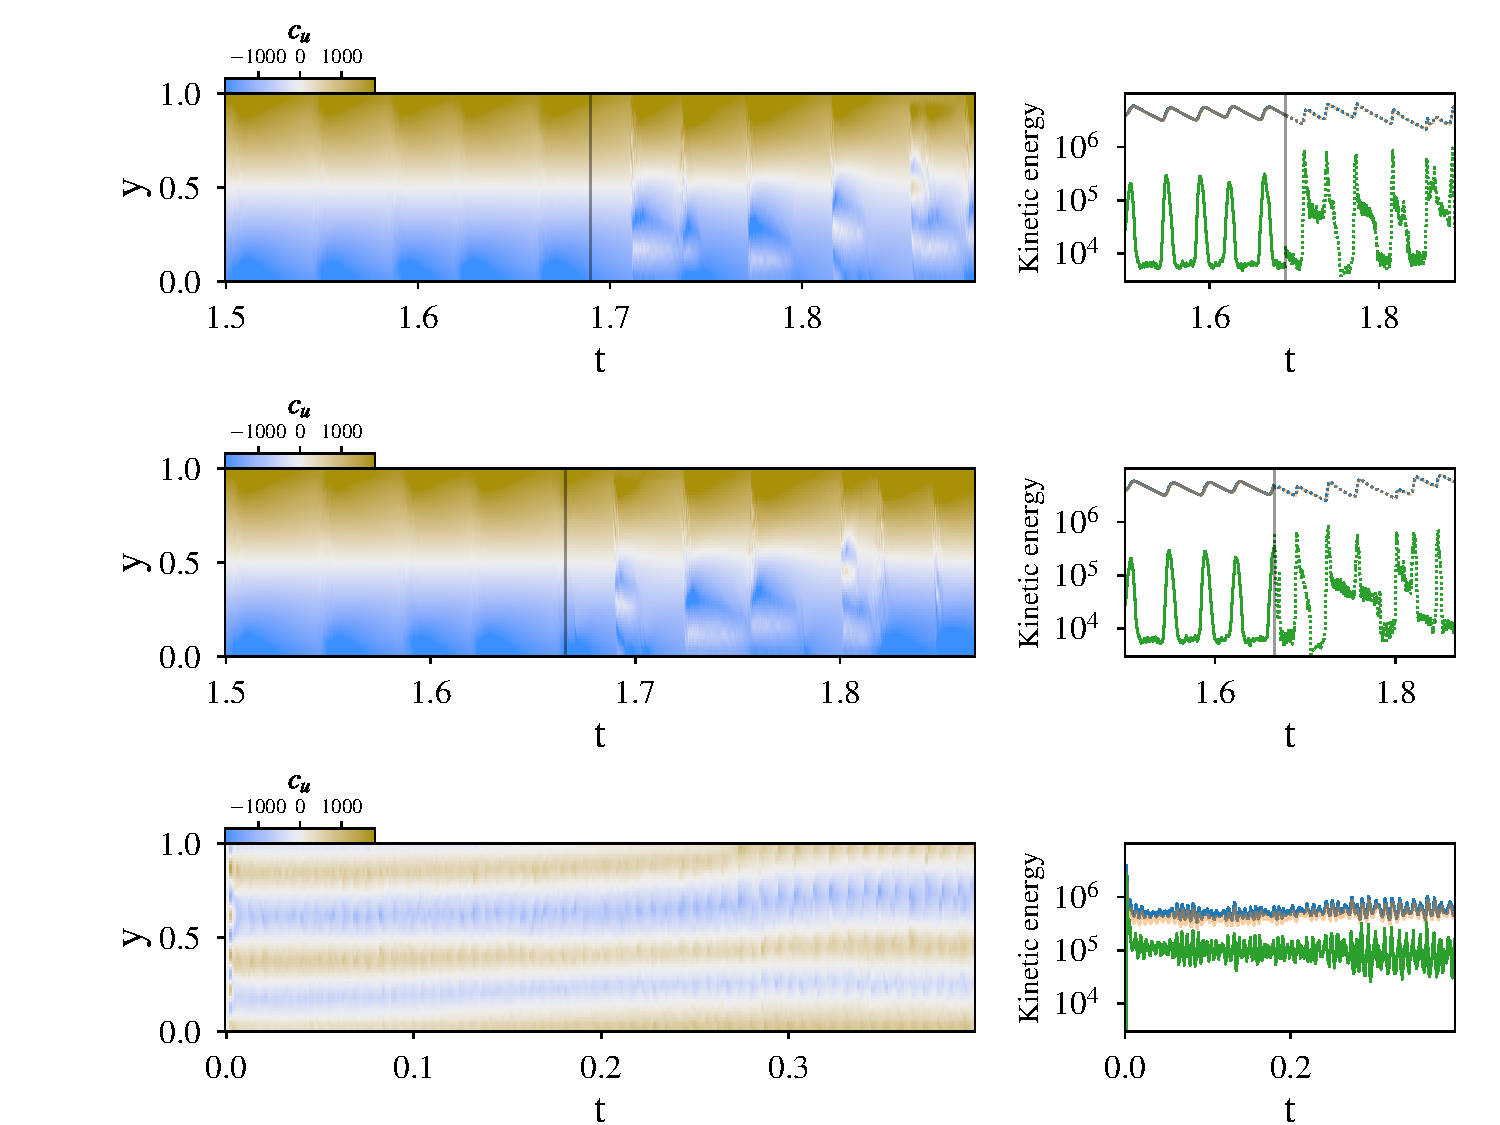
\includegraphics[width=\textwidth]{../../figs/run_C_fig.pdf}
  \caption{NOTE: timing precision of oscillator is stronger in DNS than CE2. Run C Hovmuller diagrams of $\cu$ (left) and total, zonal, and non-zonal kinetic energies (right). From top to bottom:  DNS, ``maximum knowledge'' started from bursting state of DNS solution, ``maximum ignorance'' CE2 initialized from a diagonal $\ctt$.- }
  \label{fig:run_C}
\end{figure}
%DESCRIPTION OF FIGURE 5
%\begin{itemize}
%    \item CASE C: DNS is a complicated bursting solution
%    \begin{itemize}
%        \item Predator prey type dynamics
%        \item 2 jet
%    \end{itemize}
%    \item CE2? 
%    \begin{itemize}
%        \item Biased (min ignorance) also surprisingly gives a bursting solution, slightly different characteristics but similar interactions.
%        \item biased (min ignorance). True whether started in high phase %or low phase
%        \item Unbiased system gives 5 jet solution - but still shows signs %of bursting
%    \end{itemize}
%\end{itemize}

The Busse Annulus model is capable of producing extremely complicated nonlinear spatio-temporal dynamics. Perhaps the most nonlinear behaviour exhibited by the DNS model is shown in the top panel Figure~\ref{fig:run_C}(a), which show timeseries of the total, zonal, and non-zonal kinetic energies of the flow and Hovm\"oller plots of the zonally averaged zonal flows for DNS. Here the solution takes the form of a relaxation oscillation; a cycle proceeds as follows. Convection is driven by strong temperature gradients and interacts with the rotation to generate zonal flows (in this case a two-jet solution). As more energy is pumped into the zonal flow, the shear acts so as to switch off the convection (acting as a barrier to transport). This in turn removes the energy source for the zonal flow, which decays on a longer timescale. Once the zonal flow is weak enough convection sets in again and the process is repeated. This behaviour has been described in terms of predator-prey dynamics with the convective turbulence taking the role of the prey and the zonal flows acting as a predator. 

Figure~\ref{fig:run_C}(b) shows one of the "maximum knowledge" solutions for CE2. Here the solution is started from the DNS solution when it has reached a peak in the zonal flow energy. Remarkably, CE2 is able to continue relaxation oscillations from this state; we believe that this is the first time a quasilinear model has reproduced such complicated behaviour; previous quasilinear models have been able to generate either the state at the peak or the trough of such a relaxation oscillation (REFERENCE TO PLUMMER ET AL)- but not the transition between them. If CE2 is started from the trough in the zonal flow energy, similar results are obtained (not shown). The sensitivity to initial conditions for CE2 is, however, demonstrated in Figure~\ref{fig:run_C}(c), which shows the evolution from small amplitude ``maximal ignorance" initial conditions. This solution clearly does not replicate the correct number of jets --- though it does show some indication of bursting behaviour.




%\subsection{Power Spectra}
%\label{sec:powerspec}
%Hi.



%\subsection{PDFs}
%\label{sec:pdf}

%QL pdf vs NL pdf.
%Does this do better than RB convection?

% \section{To Do}
% \label{sec:todo}

% \begin{todolist}
%   \item[\done] Fix drag runs
%     \begin{todolist}
%       \item[\done] restart a working run, adding small $C$. Does it crash?
%       \item[\done] run with each friction term off, one at a time
%     \end{todolist}
%   \item[\done] Look at 2nd cumulants
%   \item[\done] DNS with subtracted means: movie. Try to see if ``satellite modes'' are important. \textbf{Nope.}
%   \item plot DNS $k_x$ at a given height vs time.
%   \item Understand why QL/CE2 fail to reproduce correct number of jets. Is it that they can find all solutions, but cannot transition between them?
%   \item Project negative eigenvalues after run A without inline projection. Do we get the same solution? That is, are there multiple ICs that lead to similar results?
%   \item[\done] Power spectrum for $\psi$
%   \item[\done] Bias run R with 4-jet solution
%   \item[\done] Look at early time $t < 0.125$ in DNS run R. Is there a 7 jet solution present? 
%   \item Look at y-spectra for $k_x = 0$; try to see jet coalescence (maybe for paper 2) power timeseries like Bouchet et al PRL 2019?
%   \item[\done] Construct 2nd cumulants for DNS
%   \end{todolist}

%\section{Fixed points and DNS to CE2 transitions}
%\label{sec:fixed}
%Statistical methods are most illuminating when we can probe their failures as well as their successes.
%A key question is whether or not a steady-state solution of DNS is %\emph{also} a steady-state of CE2.
%In order to probe this, we computed the first and second cumulants from DNS data in three states: the steady, 2-jet solution at run A parameters, and representative burst and quiescent states from run C.

%As expected from our prior experiment in which CE2 found the same solution as DNS when biased with a high-amplitude $\cu$ initial cindition, at run A parameters, CE2 is able to continue the DNS solution easily.
%The 

%\subsection{Run C}
%\label{sec:run_c_dns_ce2}
%
%Burst and quiet.
\subsection{Rank of Second Cumulants}
\label{sec:rank}
One important difference between QL and CE2 simulations is that the former explicitly provides only a single realization of the dynamics, while the latter does not.
Recently, Nivarti et al (ADD CITATION) have shown that an important difference between the two can be quantified as the difference in the ranks of the second cumulants--that is, the number of non-zero eigenvalues they possess.
ADD MORE HERE
\begin{figure}
    \centering
    \includegraphics{}
    \caption{Caption}
    \label{fig:my_label}
\end{figure}
\section{Discussion}
\label{sec:discussion}

In this paper we have examined the effectiveness of the statistical quasilinear theory (zonally averaged CE2 --- termed zCE2) in reproducing the statistics of turbulent solutions of a model of the interaction of rotating convection and zonal flows. This Busse Annulus model exhibits complicated spatio-temporal dynamics including the formation of large-scale zonal jets, multiple zonal jets and even ``predator-prey" relaxation oscillations between states with strong zonal flows and strong convection.

We show that zCE2 is capable of reproducing even very complicated mean dynamics (such as the driving and decay of the mean flows and modification of the mean temperature profile) though, for this system, it may have multiple stable attractors for any given parameter set. If the system is initiated with \textit{maximal ignorance} then it is possible to fall into the basin of attraction of an attractor that is not preferred by DNS. It is possible to bias the symmetry of the initial condition in order to achieve solutions that mirror the symmetry of the DNS solutions. Furthermore one may use an \textit{maximal knowledge} initial condition where the zCE2 is initiated using the statistics from the saturated state of a DNS run. In this case, zCE2 appears to be extremely successful --- even reproducing the extremely nonlinear relaxation oscillations of the highly driven system.

zCE2 relies on the solution of equations for quantities averaged in the zonal direction, i.e. the mean flows and temperature and the two-point correlation functions.  It is a quasilinear theory in that the evolution equation for the two-point correlation function 
%is quasilinear in the sense that it 
is linear in the two-point correlation function, though there are terms that involve the product of the means and two-point correlation functions. The results presented here indicate that even the predator-prey dynamics is controlled by the interaction of the mean flows and temperature with the fluctuations, with the eddy/eddy $\rightarrow$ eddy nonlinearity (EENL) being of secondary importance. 

It is interesting to speculate further on the role of the missing physics encoded in the EENL. This term in the equations can be modelled by deriving evolution equations for the higher order cumulants, and truncating the hierarchy at third order. This extension to DSS is known as CE3 --- and sometimes CE2.5 when an approximate form of the CE3 equations are utilised (REF). However this is a computationally expensive procedure and solution strategies suffer severely from the ``curse of dimensionality". An interesting question then is what is the best strategy for modelling these higher-order interactions. Of course, if the linear operator provided by the mean flows and other fields is sufficiently non-normal (e.g. if for example the shear is sufficiently strong), then the precise form of this modelling term is not critical (since its role will be to act as a driving term for the non-normal modes of the linear operator). In this extreme, one may as well model these terms via delta correlated white noise. However it is possible to optimise the form of the noise provided to the linear operator so as to best match the true dynamics. Similar optimisation procedures have been utilised for the form of the (coloured) noise in transition problems (CITE JOVANOVIC AND COLLABORATORS). One strategy that appeals is to use data-driven methods to ``learn" the optimal form of the term that should be added to CE2 to best reproduce the dynamics. It is to be hoped (though by no means certain) that this optimal form should be relatively insensitive to the form of the large scales since this dependence should be encoded in the interaction between the first and second cumulants of CE2.   

PARAGRAPH BY BRAD:<< One thing that noise will do is break restricted symmetry classes, in a similar way to the EENL term. Shown by CE2.5

\bigskip


This work was supported by funding from the European Research Council (ERC) under the EU’s Horizon 2020 research and innovation programme (grant agreement D5S-DLV-786780).Computations presented here were performed on the Bates High Performance Computing Center's \emph{Leavitt} system. Computing Resources supporting this work were also provided by the NASA High-End Computing (HEC) Program through the NASA Advanced Supercomputing (NAS) Division at Ames Research Center with allocation GID s1647.
JSO was supported by NASA LWS grant No. NNX16AC92G, Research Corporation Scialog Collaborative Award (TDA) ID\#24231.


\appendix
\section{}\label{appA}
In order to ensure stability of the calculations at higher $\Rayleigh$, we have found it necessary to remove negative eigenvalues from the second cumulant at an interval of 10 timesteps.
While this is required for CE2.5 \citep{marston_qi_tobias_2019}, it appears necessary even in the CE2 simulations presented here.
The second cumulants must be positive definite in order to ensure the corresponding probability density function is realizable (that is, nowhere negative).


\bibliographystyle{jfm}
% Note the spaces between the initials
\bibliography{busse}

\end{document}

%  LocalWords:  DNS cumulants cumulant annulus
